\documentclass[qual, classic, a4paper]{ufbathesis}
\usepackage[utf8]{inputenc}
\usepackage[brazil]{babel}
\usepackage{fancyvrb}
\usepackage[alf]{abntex2cite}
\usepackage{graphicx}
\DeclareGraphicsExtensions{.pdf}

%\date{?? de Junho de 2016}
\adviser[f]{Profa. Dra. Christina von Flach G. Chavez}
\coadviser{Prof. Dr. Paulo Roberto Miranda Meirelles}

\title{
  Caracterização da qualidade interna de ferramentas de análise estática de
  código fonte
}
\author{Joenio Marques da Costa\\
  {\small joenio@joenio.me}
}

\begin{document}
\frontpage
\frontmatter
\presentationpage

%\acknowledgements
%DIGITE OS AGRADECIMENTOS AQUI
%
%\resumo
%DIGITE O RESUMO AQUI
%
%\begin{keywords}
%DIGITE AS PALAVRAS-CHAVE AQUI
%\end{keywords}
%
%\abstract
%RESUMO EM INGLÊS
%
%\begin{keywords}
%DIGITE AS PALAVRAS-CHAVE AQUI
%\end{keywords}

\tableofcontents
\listoffigures
\listoftables
\mainmatter

\chapter{Introdução}

\section{Motivação}

\begin{figure}[h]
  \center
  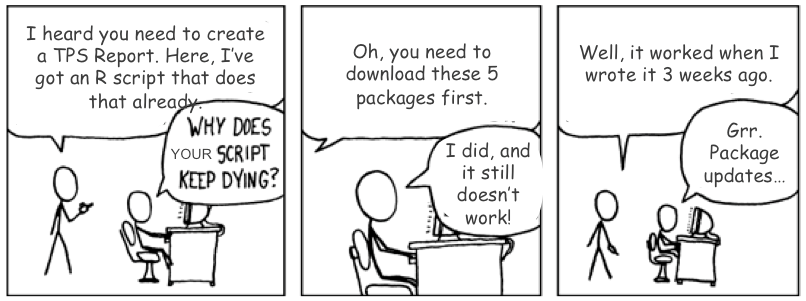
\includegraphics[scale=0.5]{imagens/reproducible-r-toolkit-cartoon.png}
  \caption{The reproducible research problem\cite{RevolutionanalyticsComRRT}}
  \label{reproducible-r-toolkit-cartoon}
\end{figure}

Reprodutibilidade é a habilidade de replicar um experimento ou estudo em sua
totalidade a fim de confirmar suas hipóteses e resultados, apesar de ser uma
prática central do método científico ainda é um grande obstáculo em muitos
estudos. Enquanto pesquisadores publicam artigos descrevendo e divulgando seus
resultados, é raro que façam o mesmo com toda a produção gerada durante a
pesquisa. A maioria dos componentes necessários para a reprodução dos
resultados de uma pesquisa na engenharia de software -- por exemplo,
código-fonte e dados -- usualmente permanecem não publicados.

Isto se configura como uma barreira para a reprodutibilidade, e
consequentemente para a repetição, replicação e variação de estudos
\cite{Feitelson2015} já que a disponibilidade de código-fonte é o mínimo
necessário para que isto ocorra \cite{Peng2011}.

Dentro deste contexto, e considerando que muitos estudos ainda sofrem com
dificuldades de repetição \cite{Tang2016}, surge a preocupação de avaliar a
qualidade dos softwares científicos a partir de métodos adequados,
especialmente em relação a sua manutenabilidade e disponibilidade por serem
problemas comuns enfrentados pelos pesquisadores \cite{Prlic2012}.

\section{Contribuições esperadas}

\begin{enumerate}
  \item Valores de referência de métricas de código-fonte para ferramentas
    de análise estática.
  \item Guia de sugestões de refatoração para ferramentas de análise estática.
  \item ...
\end{enumerate}

\chapter{Fundamentação teórica}

\section{Engenharia de Software}

Sistemas de software são utilizados em praticamente todas as áreas do
conhecimento humano e têm exercido um papel essencial em nossa sociedade
\cite{Mafra2006}. A dependência crescente de serviços oferecidos por tais
sistemas evidencia a necessidade de produzir software de qualidade,
contornando os  desafios relacionados a funcionalidades incompletas ou
incorretas, custos acima do esperado ou prazos não cumpridos.

Diante desses desafios, surge a Engenharia de Software, uma disciplina
centrada no desenvolvimento de sistemas de software através
de uma abordagem sistemática, disciplinada, e quantificável para o
desenvolvimento, operação e manutenção \cite{SWEBOK2014}.

Nas últimas décadas, o foco em estudos empíricos na área de Engenharia de
Software tem crescido significantemente \cite{Stol2015}, resultando no uso
crescente de métodos como surveys, estudos de caso, experimentos e revisões
sistemáticas de literatura. Através destes estudos empíricos, pesquisadores
transformam a Engenharia de Software em uma disciplina mais científica e
controlável -- a  Engenharia de Software Experimental -- provendo meios para
avaliar e validar métodos, técnicas, linguagens e ferramentas.

Não raro, muitos destes estudos criam novos sistemas de software, tais
sistemas costumam ser utilizados como meio para atingir os resultados da
pesquisa ou, em alguns casos, são o próprio fim do estudo realizado. Neste
trabalho, tais ferramentas de software são nosso objeto de pesquisa e serão
chamados de ``software científico'' \ -- \citeonline{Portillo12} utiliza o termo
``research tool'' para designar este mesmo tipo de software.

\subsection{Software científico}

Softwares científicos são ferramentas de software desenvolvidas no decorrer de
pesquisas científicas como parte de um estudo, podem ser pequenos scripts,
protótipos, ou mesmo produtos de software completos que demonstram ou refletem
os resultados de uma pesquisa. Em Engenharia de Software este tipo de software
desempenha um papel essencial e sua importância pode ser notada através do
grande número de conferências com sessões específicas sobre publicação de
ferramentas.

\citeonline{Kon2011} em um estudo sobre como pesquisas em Engenharia de
Software podem se beneficiar do ecosistema de Software Livre faz uma análise
de 10 edições do SBES\footnote{Simpósio Brasileiro de Engenharia de Software}
e conclui que apesar do aumento do interesse por parte dos pesquisadores em
disponibilizar o código-fonte de suas ferramentas isto ainda é minoria. O
que confirma a preocupação de \citeonline{Krishnamurthi2015} em um estudo
sobre repetibilidade de pesquisas científicas, onde chamam atenção para o papel
central que os artefatos de software possuem em pesquisas de ciência da
computação e questionam: ``Onde está o software nas pesquisas sobre linguagem
de programação?''.

A partir daí podemos afirmar que softwares científicos são peça fundamental
para que pesquisadores independentes possam reproduzir, validar ou expandir os
resultados encontrados em estudos anteriores e assim aumentar o rigor e a
qualidade científica de tais pesquisas \cite{Vitek2011}.

\subsection{Qualidade de software}

Qualidade de software diz respeito à quão bem um software é projetado e o
quanto este software está em conformidade com o projeto, embora existam
inúmeras definições há um concenso de que existem duas dimensões básicas para medir a
qualidade de um software, estas dimensões estão relacionadas à características
de qualidade interna e de qualidade externa.

Segundo \citeonline{McConnell2004}, qualidade interna são aquelas
características que preocupam o desenvolvedor, como: manutenabilidade,
flexibilidade, portabilidade, reusabilidade, legibilidade, testabilidade e
compreensão. São questões relacionadas ao código-fonte e em como o software
foi construído, como design e boas práticas por exemplo.

Qualidade externa são aquelas características que afetam o usuário, como por
exemplo: exatidão, usabilidade, eficiência, confiabilidade, integridade,
adaptabilidade, acurácia e robustez. Estas características impactam
extritamente no uso do software e não em como o software foi construído.

Segundo a ISO/IEC 25010 \cite{iso2011iec25010} essas características podem ser
divididas em subcaracterísticas. A característica usabilidade por exemplo é
dividida nas seguintes subcaracterísticas: capacidade de compreensão,
capacidade de aprendizado, operabilidade, atratividade e conformidade. Esta
característica está relacionada, por exemplo, a facilidade com que usuários aprendem e
utilizam um sistema, e passa por questões como facilidade de instalação,
aprendizado, e uso.

Sabe-se que, em algum nível, as caractarísticas de qualidade interna afetam as
características de qualidade externa \cite{McConnell2004}, softwares que não
possuem boa manutenabilidade por exemplo afetam a habilidade de correção de
defeitos, que por sua vez afetam as características de exatidão e
confiabilidade.

Dito isso podemos perceber que é possível inferir características de qualidade
externa de um software a partir de seus atributos de qualidade interna, o que
pode ser realizado a partir da análise de suas métricas de código-fonte.

\subsection{Métricas de código-fonte}

Uma métrica, segundo a definição da ISO/IEC 25010 \cite{iso2011iec25010}, é a
composição de procedimentos para a definição de escalas e métodos para
medidas, em engenharia de software estas métricas podem ser classificadas em três categorias: métricas de
produto, métricas de processo e métricas de projeto.

Métricas de produto são aquelas que
descrevem as características de artefatos do desenvolvimento, como documentos,
diagramas, código-fonte e arquivos binários. Métricas de processo medem atributos relacionados
ao ciclo de desenvolvimento do software. Métricas de projeto são aquelas
que descrevem as características dos recursos disponíveis ao desenvolvimento.

Neste trabalho, nosso interesse estão nas métricas de produto, que podem ser
classificadas entre internas ou externas, ou seja, aquelas que medem
propriedades visíveis apenas aos desenvolvedores ou que medem propriedades
visíveis aos usuários, respectivamente. Iremos extrair propriedades dos
softwares científicos a fim de medir a sua qualidade interna através de um
conjunto de métricas previamente definido, este conjunto tomará como base o
trabalho realizado por \citeonline{Meirelles2013} onde foi realizado um estudo
associando qualidade de software à qualidade de código-fonte através da
observação de métricas de código-fonte. E será realizado através de
ferramentas de análise estática de código-fonte.

\subsection{Ferramentas de análise estática de código-fonte}

Ferramentas de análise estática de código-fonte são ferramentas capazes de
realizar a leitura de código-fonte de um projeto de software de forma
automatizada ou semi-automatizada e extrair daí informações sobre as entidades
do software, como módulos, classes, funções, métodos, variáveis, seus
relacionamentos, suas características e diversas outras informações possíveis
de serem exraídas diretamente do código-fonte que seja útil ao engenheiro de
software.

Estas informaçoes costumam ser aplicadas à tarefas comuns da engenharia de
software, como por exemplo, recuperação arquitetural, localização de falhas,
manutenção, refatoração, compreensão, análise de performance, visualização,
entre outras.

Segundo \citeonline{Kirkov2010} estas ferramentas possuem uma
anatomia comum, composta de quatro componentes básicos - construção de
modelos; algoritmos de análise e reconhecimento de padrões; base de
conhecimento de padrões; e representação final.

A construção de modelos de um programa é o primeiro passo e é feito por um
parser de código-fonte \cite{Binkley2007}. A base de conhecimento de padrões é
usada para representar e armazenar informações sobre potenciais problemas
encontrados no código-fonte. O objetivo do algoritmo de análise e
reconhecumento de padroes é classificar as informações encontradas no modelo a
partir da base de conhecumento de padroes. A representação final é um
relatório ou outro tipo de visualização apresentada através de uma interface
de usuário apropriada.

Esta representação final pode ser por exemplo um relatório contendo os valores
de métricas calculadas para o software sendo analisado, e é esta
caractarística das ferramentas de análise estática de código-fonte que será
utilizada neste trabalho para recuperar métricas de produto de software que
reflitam os atributos de qualidade dos software científicos estudados.

(feedback de Paulo: faltou arrematar e contextualizar com o seu trabalho)

\section{Capítulo sobre estatística}\label{estatistica}

(ver TCC de Ronaldo e Kanashiro)

\chapter{Metodologia}

Visando então avaliar a qualidade de ``softwares científicos'' será feito um
levantamento de artigos com publicação de ferramentas do domínio {\it análise
estática de código-fonte}. Este domínio foi selecionado com base na
experiência do pesquisador nesta área, o que facilita encontrar fontes sobre
ferramentas, bem como analisar e estudar tais softwares. O foco em um domínio
se justifica pela necessidade de reduzir o escopo do estudo a fim de
viabilizar o trabalho dentro do tempo previsto em um programa de mestrado.

Além dos software científicos iremos também incluir ferramentas de análise
estática desenvolvidas na indústria, o objetivo é aumentar o número de
ferramentas analisadas visto que existe uma suspeita de encontrar um número
pequeno de softwares científicos com disponibilidade de código-fonte.

Após o levantamento e seleção das ferramentas será feita a caracterização
inicial e posteriormente análise estática do seu código-fonte, onde teremos
métricas para cada ferramenta e possivelmente valores referência para
ferramentas de análise estática, estes valores de referência darão origem a
recomendações de refatoração para ferramentas deste mesmo domínio de
aplicação.

Por final traçaremos um paralelo entre caracteristicas de qualidade externa e
valores de métricas de qualidade interna, especialmente em relação à
portabilidade e usabilidade a fim de responder nossa questão de pesquisa
e validar suas hipóteses.

%As seções à seguir descrevem em detalhes as atividades de
%cada etapa da metodologia.

\section{Questão de pesquisa e hipóteses}

A questão de pesquisa {\bf Q1} - {\it Quais características das ferramentas de
análise estática de código fonte podem ser obtidas a partir da avaliação da
sua qualidade interna?} será respondida através da validação das seguintes
hipóteses:

\begin{enumerate}
  \item[{\bf H1:}] {\em Quanto mais antiga for a publicação maior a
    probabilidade do software científico não estar mais disponível nas fontes
    indicadas}
  \item[{\bf H2:}] {\em É possível calcular valores de referência de métricas
    de código-fonte para ferramentas de análise estática a partir de um
    conjunto de softwares científicos e da indústria}
  \item[{\bf H3:}] {\em Ferramentas da indústria possuem valores de métricas
    de código-fonte mais próximos aos valores de referência do que os
    softwares científicos}
  \item[{\bf H4:}] {\em É possível relacionar a subcaracterística de qualidade
    externa operabilidade à valores de métricas de qualidade interna para os
    softwares científicos}
\end{enumerate}

% tem que explicar/justificar todas as hitóteses

A hipótese {\bf H1} será validada com a avaliação dos artigos que publicam
software científico com fontes para obtenção mas que não se encontram mais
disponíveis.

A hipótese {\bf H2} será validada (depende do capítulo \ref{estatistica}) ...

A hipótese {\bf H3} será validade a partir do cálculo das métricas de
código-fonte das ferramentas da indústria e sua comparação aos valores de
referência encontrados para as ferramentas de análise estática.

A hipótese {\bf H4} será validada com a tentativa de instalação e o uso das
funções mínimas de cada software científico avaliado, será feito a tentativa
de instalar a ferramenta, instruções de instalação e uso serão pesquisados nos
artigos relacionados bem como junto ao código-fonte do software. Espera-se que
aqueles softwares com maior dificuldade de instalação e uso terão valores de
métricas piores.

\section{Planejamento do estudo}

\subsection{Seleção das métricas}

\citeonline{Meirelles2013} realizou uma série de estudos onde associou
características de qualidade de produto de software à características de
qualidade de código-fonte, através de métricas de código-fonte, em um destes estudos
utilizou-se métricas que medem aspectos relevantes à manutenibilidade do
software, como a preocupação aqui também está na manutenibilidade
das ferramentas iremos utilizar a mesma seleção de métricas utilizada por
\citeonline{Meirelles2013}.

\begin{itemize}

  \item {\bf CBO} {\it Coupling Between Objects (Acoplamento entre objetos)}:
    mede o acoplamento entre objetos do software \cite{Chidamber1994}.

  \item {\bf LCOM4} {\it Lack of Cohesion in Methods (Ausência de coesão em
    métodos)}: mede o grau de falta de coesão em métodos \cite{Hitz1995}.

  \item {\bf SC} {\it Structural Complexity (Complexidade estrutural)}: mede a
    complexidade do software \cite{Darcy2005}.

  \item {\bf AMLOC} {\it Average Method LOC (Média do número de linhas de
    código por método)}: indica se o código está bem distribuído entre os
    métodos, quanto maior mais ``pesados'' são os métodos (??)

  \item {\bf ACCM} {\it Average Cyclomatic Complexity per Method (Média de
    complexidade ciclomática por método)}: mede a complexidade do programa
    \cite{McCabe1976}.

  \item {\bf RFC} {\it Response For a Class (Resposta para uma classe)}:
    número de métodos dentre todos os métodos que podem ser invocados em
    resposta a uma mensagem enviada por um objeto de uma classe
    \cite{Sharble1993}.

  \item {\bf DIT} {\it Depth of Inheritance Tree (Profundidade da árvore de
    herança)}: mede o número de ancestrais de uma classe \cite{Shih1997}.

  \item {\bf NOC} {\it Number Of Children (Número de filhos)}: número total de
    filhos de uma classe \cite{Rosenberg1997}.

  \item {\bf COF} {\it Coupling Factor (Fator de acoplamento)}: razão entre o
    número máximo possível de acoplamentos no sistema e o número atual de
    acoplamentos possíveis por herança \cite{Harrison1998}.

\end{itemize}

Estas métricas serão coletadas para cada classe/módulo presente nas
ferramentas de análise estática selecionadas e servirão de base para
avaliar a qualidade das mesmas.

\subsection{Seleção da ferramenta de análise estática de código-fonte}

Para realizar a caracterização das ferramentas e extrair suas métricas
será necessário uma ferramenta que permita automatizar este
processo, neste trabalho utilizaremos a ferramenta de análise estática Analizo
\cite{Terceiro2010}.

Analizo é um {\it toolkit} livre, multi-linguagem e extensível para análise de
código-fonte, calcula uma grande quantidade de métricas, como CBO, LCOM4, RFC,
LOC, entre outras, e suporta análise das linguagens de programação C, C++ e
Java.

É uma ferramenta mantida constantemente, com desenvolvedores ativos, e
atualizações frequentes, sua última versão 1.19.0 lançada em 18 de Fevereiro
de 2016 será a versão utilizada neste estudo.

%eu sou um dos desenvolvedores dessa ferramenta o que me dá a
%capacidade de realizar atualizações ou correção de problemas ao longo deste
%estudo caso isto venha a ser necessário.

\subsection{Seleção das fontes de ferramentas de análise estática}\label{levantamento}

Para ser possível validar as hipóteses aqui levantadas é necessário realizar
uma busca por ferramentas de análise estática desenvolvidas no contexto da
academia e da indústria, para isso, será feito um planejamento detalhado para
realizar a seleção de ferramentas em cada um destes contextos.

No contexto acadêmica a busca por ferramentas será feita
através de artigos publicados em conferências que tenham histórico de
publicação sobre ferramentas de análise estática de código fonte. Estes
artigos serão analisados e aqueles com publicação de ferramenta de análise
estática serão selecionados.

Na indústria, a busca por ferramentas será feita a partir
de referências encontradas na internet, algumas organizações mantém listas de
ferramentas para análise de código-fonte, a Wikipedia por exemplo, mantém uma lista
de ferramentas, estas referências serão utilizadas como ponto de partida e
cada ferramenta será analisada a fim de validar se são da indústria ou
surgiram em contexto acadêmico.

Uma vez que as ferramentas tenham sido selecionadas iniciaremos a extração de
seus atributos de qualidade interna a partir do cálculo de suas métricas com o
Analizo.

\section{Coleta de dados}

A partir das fontes selecionadas na etapa anterior serão realizadas duas
atividades para identificar e mapear as ferramentas de análise estática com
código-fonte disponível, uma atividade relacionada ao levantamento de
ferramentas da academia, outra atividade relacionada ao levantamento de
ferramentas da indústria.

\subsection{Ferramentas da academia}

A seleção de ferramentas será relizada através de uma revisão estruturada dos
artigos selecionados a partir das seguintes conferências:

\begin{itemize}
  \item ASE - Automated Software
    Engineering\footnote{http://ase-conferences.org}
  \item CSMR\footnote{A conferência CSMR tornou-se SANER - Software Analysis,
    Evolution, and Reengineering a partir da edição 2015.} - Conference on
    Software Maintenance and
    Reengineering\footnote{http://ansymore.uantwerpen.be/csmr-wcre}
  \item SCAM - Source Code Analysis and Manipulation Working
    Conference\footnote{http://www.ieee-scam.org}
  \item ICSME - International Conference on Software Maintenance and
    Evolution\footnote{http://www.icsme.org}
\end{itemize}

Chamamos de revisão estruturada um processo disciplinado para seleção de
artigos a partir de critérios bem definidos de forma que seja possível a
reprodução do estudo por parte de pesquisadores interessados. Alguns
resultados preliminares podem ser consultados na Tabela \ref{artigos-do-scam}
da Seção \ref{resultados}.

\subsection{Ferramentas da indústria}

A seleção de ferramentas da indústria será feita de forma não estruturada a
partir de uma busca livre e manual em fontes encontradas na Internet sobre
ferramentas de análise estática. Nos estudos já realizados as seguintes fontes
foram selecionadas:

\begin{itemize}

  \item Projeto SAMATE\footnote{http://samate.nist.gov} - {\em Software
    Assurance Metrics and Tool Evaluation} disponível em
    \citeonline{SamateAnalysers} mantém uma lista de ferramentas de análise
    estática, detalhes sobre o projeto pode ser encontrado em
    \citeonline{Ribeiro2015}.

  \item O software Spin mantém em seu site uma lista de ferramentas comerciais
    e de pesquisa para análise estática de código-fonte para C em
    \citeonline{spinSourceAnalysisTools}.
    
  \item O Instituto de Engenharia de Software do CERT mantém uma lista de
    ferramentas de análise estática em \citeonline{certSecureCodingTools}.
    
  \item O software Flawfinder oferece em seu site um link com referências para
    inúmeras ferramentas livres, proprietárias e gratuitas de ferramentas de
    análise estática e outros tipos de análise em
    \citeonline{wheelerStaticAnalysisTools}.

  \item Uma outra fonte contendo uma relação expressiva de ferramentas é
    mantida na Wikipedia em \citeonline{wikipediaListStaticCodeAnalysis}.

\end{itemize}

Estas fontes serão pesquisadas manualmente em busca de ferramentas de análise
estática que tenham sido desenvolvidas no contexto da indústria, alguns
resultados preliminares podem ser encontrados nas Tabelas
\ref{ferramentas-do-nist-com-codigo} e \ref{ferramentas-do-nist-sem-codigo}.

\subsection{Caracterização dos artigos}

Os artigos selecionados a partir da revisão estruturada serão avaliados a fim
de caracterizar se se tratam de publicação de ferramenta de análise estática
de código-fonte, esta revisão será realizada de forma semi-automatizada, o
primeiro passo será automatizado a partir de um
script\footnote{http://github.com/joenio/dissertacao-ufba-2016/blob/master/revisao-estruturada/filter}
que busca os seguintes termos no conteúdo dos artigos:

\begin{verbatim}
  "tool" OU "framework"; E
  "download" OU "available"; E
  "http" OU "ftp"; E
  "static analysis" OU "parser".
\end{verbatim}

O segundo passo, manual, é realizar uma leitura do artigo a fim de identificar
se realmente trata-se de um artigo com publicação de {\it software
científico}, uma vez que se confirme que o artigo publica um software,
identifica-se se o software é uma ferramenta de análise estática, softwares
que sejam mais abrangentes do que apenas análise estática mas que contenham
esta função em seu conjunto também será considerados.

Uma vez identificado os artigos que publicam {\it softwares científicos} de
análise estática, procuramos no próprio artigo referências de onde encontrar o
software, neste momento algumas ações serão tomadas a partir da situação
encontrada.

\begin{itemize}

  \item Aqueles autores que afirmam que a ferramenta está disponível mas o
    artigo não cita referências de onde encontrar serão contactados por email
    solicitando informações de onde obter o código-fonte.

  \item Os artigos que indicam onde obter o cófigo-fonte mas o acesso ao local
    indicado não está disponível, ou está disponível mas o software não se
    encontra lá, os autores também serão contactados solicitando informações
    atualizadas de onde obter uma cópia do código-fonte da ferramenta

  \item Os demais artigos que indicam onde obter o cófigo-fonte e a referência
    está correta, iremos fazer downlod da última versão disponível do software

\end{itemize}

Uma vez que os autores contactados por email respondam com informações de onde
obter o software iremos adicinar estes softwares na lista de softwares a serem
analisados.

\subsection{Caracterização das ferramentas}

As ferramentas da indústria e acadêmicas serão analisadas com o Analizo para
extração das métricas de código-fonte préviamente
selecionadas, estas métricas serão relacionadas à caractarística e atributos
de qualidade das ferramentas.

As métricas coletadas serão também utilizadas para identificar se existem
valores de referência para métricas de ferramentas de análise estática, caso
existam, estes valores de métricas serão utilizadas para calcular quão
distante cada ferramenta analisada se encontra dos valores de referência, isto
será feito com base no trabalho realizado \citeonline{Ronaldo2015} onde o
mesmo estudo foi feito para o sistema Android e seus aplicativos.

\section{Exemplo de uso}

Por fim, os valores de referência encontradas serão documentados e servirão de
base para criar um guia de sugestões para refatoração de ferramentas de
análise estática. Tomaremos como exemplo de uso a própria ferramenta Analizo,
onde iremos calcular suas métricas e a partir de uma comparação com os
valores de referência indicaremos refatorações que façam a ferramenta de
aproximar dos valores de referência.

Estas indicações serão feitas utilizando o mesmo método de
\citeonline{Almeida2010} onde foi feito um estudo mapeando boas práticas de
programação em valores de métricas de código-fonte, estas boas práticas são
baseadas nos trabalhos de \cite{Martin2012} e \cite{Beck2007} sobre {\it Clean
Code}, onde sugerem práticas de desenvolvimento úteis para que um código
tenham expressividade, simplicidade e flexibilidade. Neste trabalho os autores
identificam melhorias de implementação através do uso de valores de métricas e
oferecem aos desenvolvedores uma maneira de pensarem em melhorias para os seus
códigos.

\chapter{Análise}

\section{Resultados preliminares}\label{resultados}

A Tabela \ref{artigos-do-scam} apresenta um resumo do número de artigos em
cada edição do SCAM e quantos artigos trazem publicação de ferramenta de análise
estática com código fonte disponível.

\begin{table}
\caption{Total de artigos analisados por edições do SCAM}
\centering
\begin{tabular}{| l | c | c | c |}
\hline
Edição    & Total de artigos & Script filter & Artigos com ferramenta \\
\hline
SCAM 2001 & 23               & 6             & -                      \\
SCAM 2002 & 18               & 6             & -                      \\
SCAM 2003 & 21               & 7             & -                      \\
SCAM 2004 & 17               & 3             & -                      \\
SCAM 2005 & 19               & 7             & -                      \\
SCAM 2006 & 22               & 9             & 2                      \\
SCAM 2007 & 23               & 7             & 1                      \\
SCAM 2008 & 29               & 14            & -                      \\
SCAM 2009 & 20               & 10            & -                      \\
SCAM 2010 & 21               & 15            & 1                      \\
SCAM 2011 & 21               & 9             & 1                      \\
SCAM 2012 & 22               & 12            & 4                      \\
SCAM 2013 & 24               & 12            & -                      \\
SCAM 2014 & 35               & 16            & 1                      \\
SCAM 2015 & 30               & 18            & ?                      \\
\hline
Total     & 315              & 133           & 10                     \\
\hline
\end{tabular}
\label{artigos-do-scam}
\end{table}

As Tabelas \ref{ferramentas-do-nist-com-codigo} e
\ref{ferramentas-do-nist-sem-codigo} apresentam ferramentas do NIST após
avaliação inicial sobre disponibilidade do código-fonte. Das 54 ferramentas
apenas 19 tinham código fonte disponível.

% Todos foram baixados em "dataset/NIST".

\begin{table}
\caption{Lista de ferramentas do SAMATE - NIST com código fonte não disponível}
\centering
\begin{tabular}{| l | l |}
\hline
Ferramenta & Avaliacao  \\
\hline
ABASH                     & código não disponível \\
ApexSec Security Console  & código não disponível \\
Astrée                    & código não disponível \\
bugScout                  & código não disponível \\
C/C++test®                & código não disponível \\
dotTEST™                  & código não disponível \\
Jtest®                    & código não disponível \\
HP Code Advisor (cadvise) & código não disponível \\
Checkmarx CxSAST          & código não disponível \\
CodeCenter                & código não disponível \\
CodePeer                  & código não disponível \\
CodeSecure                & site offline \\
CodeSonar                 & código não disponível \\
Coverity SAVE™            & código não disponível \\
Csur                      & código não disponível \\
DoubleCheck               & código não disponível \\
Fluid                     & código não disponível \\
Goanna Studio and Goanna Central & código não disponível \\
HP QAInspect              & código não disponível \\
Insight                   & código não disponível \\
ObjectCenter              & código não disponível \\
Parfait                   & código não disponível \\
PLSQLScanner 2008         & código não disponível \\
PHP-Sat                   & link para código offline \\
PolySpace                 & código não disponível \\
PREfix and PREfast        & código não disponivel \\
QA-C, QA-C++, QA-J        & código não disponível \\
Qualitychecker            & código não disponível \\
Rational AppScan Source Edition & código não disponível \\
Resource Standard Metrics (RSM) & código não disponível \\
SCA                       & código não disponível \\
SPARK tool set            & código não disponível \\
TBmisra®, TBsecure®       & código não disponível \\
PVS-Studio                & código não disponível \\
xg++                      & código não disponível \\
\hline
\end{tabular}
\label{ferramentas-do-nist-sem-codigo}
\end{table}

\begin{table}
\caption{Lista de ferramentas do SAMATE - NIST com código fonte disponível}
\centering
\begin{tabular}{| l | l |}
\hline
Ferramenta & Avaliacao  \\
\hline
BOON                      & código disponível \\
Clang Static Analyzer     & código disponível \\
Closure Compiler          & código disponível \\
Cppcheck                  & código disponível \\
CQual                     & código disponível \\
FindBugs                  & código disponível \\
FindSecurityBugs          & código disponível \\
Flawfinder                & código disponível \\
Jlint                     & código disponível \\
LAPSE                     & código disponível \\
Pixy                      & código disponível \\
PMD                       & código disponível \\
pylint                    & codigo disponivel \\
RATS (Rough Auditing Tool for Security) & código disponível \\
Smatch                    & código disponível \\
Splint                    & código disponível \\
UNO                       & código disponível \\
Yasca                     & código disponível \\
WAP                       & código disponível \\
\hline
\end{tabular}
\label{ferramentas-do-nist-com-codigo}
\end{table}

Assim, temos um total de 19 ferramentas da indústria com código-fonte
disponível e ??? da academia com código fonte disponível, é preciso avaliar em
qual linguagem de programação foi escrita cada ferramentas pois só iremos
analisar aquelas em C, C++ ou Java que são suportadas pelo Analizo.

A ferramenta utilizada para identificar a linguagem de programação em que
estes softwares foram escritos foi a sloccount, uma ferramenta livre para
contagem de linhas de código fonte, onde se calcula em quais linguagens de
programação um software foi escrito.

%Abaixo destaco a linguagem de programação que tem maior
%porção em porcentagem.

Após analise ficamos com um total de 25 ferramentas, 15 da indústria e 10 da
academia, a Tabela \ref{total-de-ferramentas} traz um resumo de todos as
ferramentas analisadas.

\begin{table}
\caption{Lista com total de ferramentas a serem analisadas}
\centering
\begin{tabular}{| l | c | c |}
\hline
Ferramenta & Linguagem & Fonte \\
\hline
BOON                  & ansic                & industria \\
CQual                 & ansic                & industria \\
RATS                  & ansic                & industria \\
Smatch                & ansic                & industria \\
Splint                & ansic                & industria \\
UNO                   & ansic                & industria \\
Clang Static Analyzer & cpp                  & industria \\
Cppcheck              & cpp                  & industria \\
Jlint                 & cpp                  & industria \\
WAP                   & java                 & industria \\
Closure Compiler      & java                 & industria \\
FindBugs              & java                 & industria \\
FindSecurityBugs      & java                 & industria \\
Pixy                  & java                 & industria \\
PMD                   & java                 & industria \\
Indus                 & java                 & academia  \\
TACLE                 & java                 & academia  \\
JastAdd               & java                 & academia  \\
WALA                  & java                 & academia  \\
error-prone           & java                 & academia  \\
AccessAnalysis        & java                 & academia  \\
Bakar Alir            & java/ada/python      & academia  \\
InputTracer           & ansic                & academia  \\
srcML                 & cpp/cs (cs = C\# ?)   & academia  \\
Source Meter          & java                 & academia  \\
\hline
\end{tabular}
\label{total-de-ferramentas}
\end{table}

\chapter{Conclusão}

(à fazer)

\backmatter
\appendix
\bibliography{bibliografia}
\end{document}
